\chapter{Propuesta de Investigación}
\label{sec:propuesta}

\section{Planteamiento del problema}

Desde sus principios, los sistemas de posicionamiento satelital han sido construidos con el único propósito de contar con una herramienta tecnología que permita localizar un receptor de señal GPS en casi cualquier lugar del mundo, en cualquier momento. Es así como desde sus inicios en 1960 sistema de posicionamiento global GPS creado por el DOD\footnote{DoD: Departamento de estado de los Estados Unidos de Norteamérica}, fue enfocado a tareas de alta precisión como herramienta estratégica para tareas militares.\\

Aunque el diseño detrás los sistemas satelitales, toma en cuenta un gran número de variables y fenómenos físicos involucrados en el funcionamiento de este tipo de sistemas, el nivel de precisión está ligado a las características del medio en el cual viajan las señales (ionosfera, troposfera)\cite{Hofmann_Wellenhof_1992}, limitantes propias del hardware en satélites y receptores (errores en sincronización de reloj) y otras fuentes de error mas difíciles de sortear aún, como los efectos relativistas, precidicción del ciclo solar, etc. \cite{de2007analise}, \cite{Novatel:2015:Online}.\\%(ref sobre los errores que aquejan GNSS y la precisión)\\

Uno de los principales problemas de los sistemas de navegación basados en GNSS es la degradación de la precisión cuando alguno de los satélites es bloqueado, como es el caso de los edificios dentro del ambiente urbano, la vegetación espesa en zona selvática o fenómenos de interferencia entre las señales que llegan al receptor.\\

Por otra parte, se ha venido observando en los recientes estudios de estabilidad en sistemas satelitales que a medida que la cantidad de satelites disponibles aumenta la ocurrencia de fallos en la sincronización de reloj también aumenta. El segmento de control GNSS es el encargado de monitorear y marcar los satelites que presentan errores de sincronización o estan defasados de orbitas; de esta forma estos satélites no son aptos para una buena precisión en posicionamiento.\\
% Basado en las patentes 
%	http://www.google.com/patents/US20140232595
%	https://www.google.ch/patents/US9170109

En este orden de ideas, las técnicas de posicionamiento muestran ser muy robustas en condiciones de estáticas y con buena visibilidad, la navegación dentro de las ciudades impone unas condiciones diferentes, bajo las cuales solo un monto de todos los satélites es visible.
%lo que conlleva a tener mayor imprecisión en el posicionamiento debido a una mayor cantidad errores inducidos en las señales satelitales recibidas.\\ % Cooperative GPS/INS Navigation in Urban Enviroment Berefelt, Boberg ZZZ 2004

Por ello se ha venido considerando importante el desarrollar nuevos algortimos y técnicas de posicionamiento para su uso dentro de ambientes urbanos, tras el objetivo de alcanzar mayores niveles de precisión dentro de ambientes urbanos.\\

Una buena parte de los reportes de literatura durante la ultima década han sido enfocados a caracterizar la precisión de GPS y GNSS en ambientes a cielo abierto y urbanos, empleando dispositivos de posicionamiento estáticos. En en estos reportes se hace énfasis en el impacto que tienen la baja visibilidad de satelitales, interferencia inter-canal y el obstrucción de señales, como los factores que impiden alcanzar mayores niveles de precisión en dispositivos GPS inmersos en cañones urbanos.\\ 

Cuando se tiene en cuenta que para 2020 habrá una gran infraestructura satelital disponible, que el mercado de los dispositivos electrónicos actual ofrece una variedad de dispositivos para la recepción de señales GPS, así también, tecnologías y módulos embebidos que posibilitan la interconexión entre dispositivo; surge la idea que da origen a la presente investigación bajo la pregunta: \\

%Por ello se considera relevante abordar el presente estudio, apoyado en la pregunta de investigación: \\

\begin{example}{Pregunta de investigación}
¿Es posible contribuir a la mejora del nivel de precisión en posicionamiento dentro de ambientes urbanos, mediante la interacción de dispositivos GPS?\\
\end{example}

El buscar una alternativa de respuesta a la pregunta anterior, es la principal motivación para llevar a cabo la presente investigación, bajo la siguiente hipótesis:\\

\begin{example}{Hipótesis}
Desarrollar una técnica de posicionamiento para cañones urbanos basada en interacción de dispositivos GPS, podría permitir que estos dispositivos entre sí se beneficien de la información satelital adquirida por sus semejantes para mejorar su nivel de precisión en posicionamiento.
\end{example}


En calidad de abordar la búsqueda de precisión en sistemas de posicionamiento inmersos en ambientes urbanos, se ha realizado un breve recorrido por la literatura el cual será presentado en la sección \ref{sec:estadodelarte}.\\

%########################################################################
%########################################################################
\section{Justificación}

Tras la meta de reducir los costos y mejorar la precisión en posicionamiento de los receptores GPS y/o GNSS, han surgido desarrollos de software que implementan las tareas de hardware por medio de funciones de software. Este tipo de librerías y paquetes de software se les conoce como radio definido por software (SDR) y se ha hecho popular durante de la pasada década \cite{Goodman_2003}, \cite{Petovello_2008}. Algunas librerías como RTKLIB\cite{takasu2008evaluation} y GPSTk\cite{ion:gnss04}, facilitan las tareas de adquisición y procesamiento de datos desde los dispositivos y módulos GPS.\\

Por ello se considera que el uso de este tipo de herramientas de software y la apropiación del conocimiento detrás de la tecnología GPS/GNSS, permitiría el desarrollo de la idea de investigación planteada en la presente propuesta, que aportarían a la planificación urbanística de la ciudad de bucaramanga con miras a su futura transformación en ciudad inteligente; donde se pueda contar con con sistemas de transporte urbano inteligentes o la planificación vial urbana, como podría ser el caso de la infraestructura vial enmarcada dentro del proyecto regional Diamante Santander-Caribe.\\

En la figura extraída desde la publicación de \cite{laurini2002information}, se presenta de forma clara el impacto que puede tener la precisión de los sistemas de posicionamiento para otras aplicaciones e intereses dentro de la planificación urbana y departamental.

\begin{figure}[htbp]
	\centering
	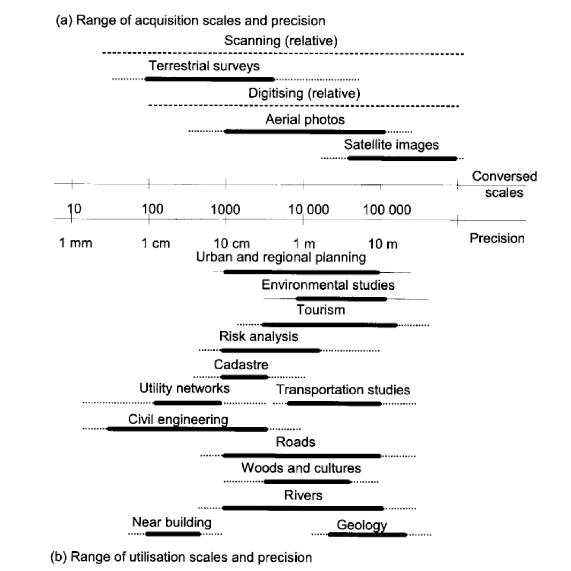
\includegraphics[scale=0.58]{Imagenes/Apps.png}
	\caption{Escala de adquisición de los datos y principales usos. a) Rango de adquisición vs Escala b) Rango de Utilización vs Escala. \cite{laurini2002information}} 
	\label{fig:Apps}
\end{figure}


Además los resultados obtenidos de la presente investigación pueden contribuir al fortalecimiento de las líneas de investigación en las áreas de sistemas embebidos, sistemas de comunicaciones e ingeniería del software en la Universidad Industrial de Santander. \\

%########################################################################
%########################################################################
%\section{Motivación}


